\section{Metodología}

El proyecto se lleva a cabo siguiendo varias etapas clave que cincluyen la investigación, el diseño, la construcción y la prueba del mecanismo. Cada etapa se desarrolla de manera sistemática para garantizar que se cumplan los objetivos del proyecto y se obtengan resultados significativos. 

Concluida la etapa de investigación, a continuación se detallan las siguientes etapas de la metodología empleada:

\subsection{Diseño del mecanismo}

El diseño del mecanismo \textit{Theo Jansen} se basa en los principios de la mecánica clásica y la cinética. Las partes importantes del mecanismo incluyen:

\begin{itemize}
  \item \textbf{Ejes y engranajes:} Estos componentes son fundamentales para transmitir el movimiento del viento al mecanismo. Los ejes permiten que las partes móviles giren, mientras que los engranajes ayudan a convertir el movimiento rotacional en movimiento lineal, lo que es esencial para el funcionamiento del mecanismo.
  \item \textbf{Estructura de soporte:} La estructura del mecanismo debe ser lo suficientemente robusta para soportar las fuerzas generadas por el viento y el movimiento del mecanismo y al mismo tiempo ser lo suficientemente ligera para permitir que el viento la mueva. Esto se logra mediante el uso de materiales adecuados y un diseño estructural eficiente.
  \item \textbf{Articulaciones:} Se refiere a las conexiones entre las diferentes partes del mecanismo que permiten el movimiento relativo entre ellas. Estas articulaciones son cruciales para garantizar que el mecanismo funcione de manera fluida y eficiente.
\end{itemize}

Una de las partes fundamentales, luego de diseñar estos componentes, son las patas del mecanismo, que permiten que se mueva y camine de manera eficiente y fluida, según el creador del mecanismo, Theo Jansen. Este simula el movimiento de la pata de un animal y ha sido perfeccionado durante los últimos 10 años mediante un algoritmo evolutivo. Según \textit{Bustamante T. (2016)}, el criterio principal para el desarrollo de estas patas es el rendimiento de los elementos en la tarea encomendada, utilizando los errores y mejoras de las evoluciones para optimizar el diseño en cada iteración. \cite{tellez2016diseno}

Este algoritmo evolutivo entrega al final de sus múltiples iteraciones las medidas de las patas del mecanismo, lo que su creador denomina \textbf{\textit{Los números sagrados}}

\begin{table}[H]
  \centering
  \caption{Valores asignados a cada letra}
  \begin{tabular}{cc|cc}
    \toprule
    \textbf{Letra} & \textbf{Valor} & \textbf{Letra} & \textbf{Valor} \\
    \midrule
    a & 38.0 & g & 36.7 \\
    b & 41.5 & h & 65.7 \\
    c & 39.3 & i & 49.0 \\
    d & 40.1 & j & 50.0 \\
    e & 55.8 & k & 61.9 \\
    f & 39.4 & l & 7.8 \\
    \multicolumn{4}{c}{\textbf{m = 15.0}} \\
    \bottomrule
  \end{tabular}
\end{table}

Estos valores hacen posible un movimiento fluido y áltamente eficiente del mecanismo, permitiendo que se mueva con la energía cinética del viento.

De acuerdo a esta lista es necesario poder escalar las medidas de las patas del mecanismo para que se ajusten a las dimensiones del proyecto. Para ello, se establece un factor de escala que es la relación entre las dimensiones del mecanismo y las dimensiones reales de las patas.

Como medida base se toma la longitud más grande \textbf{h} que pretende ser de 65.7 cm pero se escalará a 21.5 cm de acuerdo a la siguiente expresión:
\begin{equation}
  \text{Factor de escala} = \frac{\text{Longitud deseada}}{\text{Longitud original}} = \frac{21.5}{65.7} \approx 0.33
\end{equation}

Es entonces de acuerdo a este factor de escala que se multiplicarán las medidas de las patas del mecanismo para obtener las dimensiones reales de las patas del mecanismo obteniendo así las longitudes entre ejes de rotación de las articulaciones que se usarán para el proyecto. A continuación se muestran las medidas escaladas de las patas del mecanismo \textit{Theo Jansen} y al costado el margen de medio centímetro en cada extremo que asegura espacio para las uniones de las patas con los ejes de rotación:

\begin{multicols}{2}
  \begin{table}[H]
    \centering
    \caption{Longitud entre ejes de rotación}
    \begin{tabular}{cc|cc}
      \toprule
      \textbf{Letra} & \textbf{Valor} & \textbf{Letra} & \textbf{Valor} \\
      \midrule
      a & 12.5 & g & 12.1 \\
      b & 13.7 & h & 21.7 \\
      c & 13.0 & i & 16.2 \\
      d & 13.2 & j & 16.5 \\
      e & 18.4 & k & 20.4 \\
      f & 13.0 & l & 2.6 \\
      \multicolumn{4}{c}{\textbf{m = 5}} \\
      \bottomrule
    \end{tabular}
  \end{table}
  
  \begin{table}[H]
    \centering
    \caption{Longitud completa con margen}
    \begin{tabular}{cc|cc}
      \toprule
      \textbf{Letra} & \textbf{Valor} & \textbf{Letra} & \textbf{Valor} \\
      \midrule
      a & 13.5 & g & 13.1 \\
      b & 14.7 & h & 22.7 \\
      c & 14.0 & i & 17.2 \\
      d & 14.2 & j & 17.5 \\
      e & 19.4 & k & 21.4 \\
      f & 14.0 & l & 3.6 \\
      \multicolumn{4}{c}{\textbf{m = 6}} \\
      \bottomrule
    \end{tabular}
  \end{table}
\end{multicols}

Una vez encontradas estas medidas se pretenden ensamblar de la siguiente manera:
\begin{figure}[H]
  \centering
  \caption{Diagrama de las patas del mecanismo \textit{Theo Jansen} con los números sagrados} 
  \label{fig:diagrama_barras}
  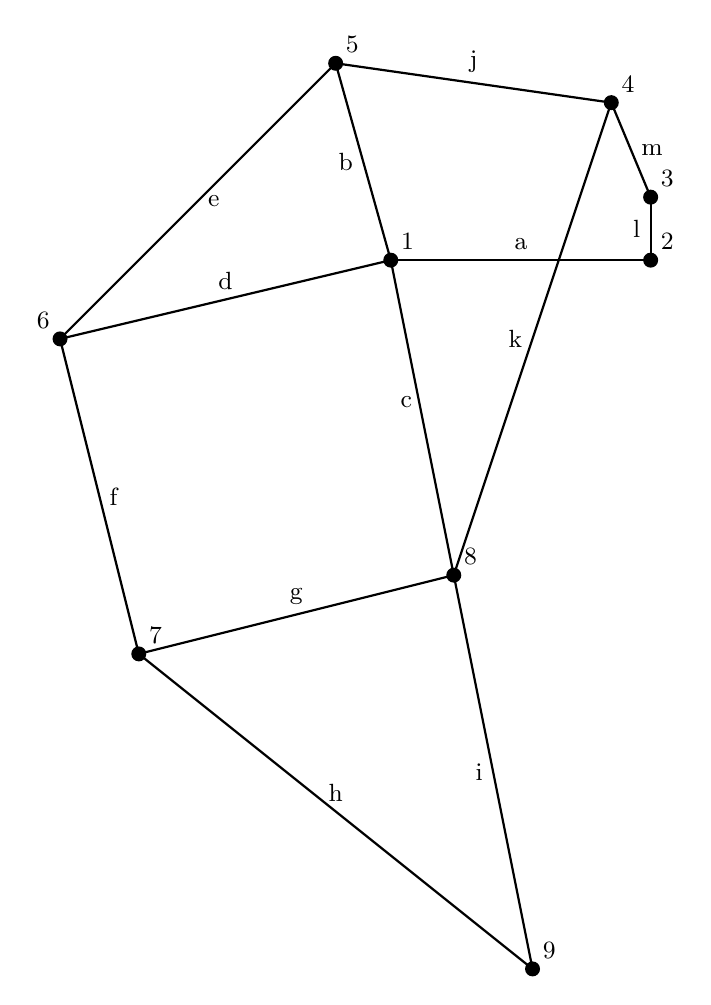
\begin{tikzpicture}[scale=0.1, thick, every node/.style={scale=1}]

  \coordinate (P1) at (22,30);
  \coordinate (P2) at (55,30);
  \coordinate (P3) at (55 ,38);
  \coordinate (P4) at (50,50);
  \coordinate (P5) at (15,55);
  \coordinate (P6) at (-20,20);
  \coordinate (P7) at (-10,-20);
  \coordinate (P8) at (30,-10);
  \coordinate (P9) at (40,-60);

  \draw (P1) -- (P2) node[midway,above] {\small a};
  \draw (P2) -- (P3) node[midway,left] {\small l};
  \draw (P3) -- (P4) node[midway,right] {\small m};
  \draw (P4) -- (P5) node[midway,above] {\small j};
  \draw (P5) -- (P1) node[midway,left] {\small b};
  \draw (P5) -- (P6) node[midway,right] {\small e};
  \draw (P6) -- (P1) node[midway,above] {\small d};
  \draw (P6) -- (P7) node[midway,right] {\small f};
  \draw (P1) -- (P8) node[midway,above left] {\small c};
  \draw (P7) -- (P8) node[midway,above] {\small g};
  \draw (P7) -- (P9) node[midway,above] {\small h};
  \draw (P9) -- (P8) node[midway,left] {\small i};
  \draw (P8) -- (P4) node[midway,left] {\small k};
  
  \filldraw (P1) circle (23pt) node[above right] {\small 1};
  \filldraw (P2) circle (23pt) node[above right] {\small 2};
  \filldraw (P3) circle (23pt) node[above right] {\small 3};
  \filldraw (P4) circle (23pt) node[above right] {\small 4};
  \filldraw (P5) circle (23pt) node[above right] {\small 5};
  \filldraw (P6) circle (23pt) node[above left] {\small 6};
  \filldraw (P7) circle (23pt) node[above right] {\small 7};
  \filldraw (P8) circle (23pt) node[above right] {\small 8};
  \filldraw (P9) circle (23pt) node[above right] {\small 9};
  \end{tikzpicture}
\end{figure}


\subsection{Materiales}

Dentro del marco del proyecto, se emplean diversos materiales para la construcción del mecanismo \textit{Theo Jansen}. Estos materiales son seleccionados fueron esocgidos por su durabilidad, flexibilidad y ligeresa, lo que permite que el mecanismo funcione de manera eficiente y efectiva. Los materiales utilizados incluyen:

\begin{itemize}
  \item \textbf{Sorbetes de plástico:} Estos sorbetes son utilizados para las patas del mecanismo, ya que son ligeros y flexibles, lo que permite que el mecanismo se mueva de manera eficiente. Además, los sorbetes son fáciles de conseguir y económicos, lo que los convierte en una opción ideal. Además de ser increíblemente resistentes ante la presión y torsión.
  
  \item \textbf{Hilo de coser o pavilo:} Este hilo se utiliza para unir las diferentes partes de la pata, hacen posible rotar a la articulación de manera que no es afectada por la fricción.
  
  \item \textbf{Palillos de manera:} Es importante fijar las patas a un eje central, para lo cual se utilizan palillos de madera. Estos palillos son resistentes y permiten unir las patas mediante el cigüeñal del mecanismo que convertirá el movimiento rotacional en movimiento lineal.
  
  \item \textbf{Palillos de fosforos:} Estos palillos se utilizan para la misma función que el hilo.
  
  \item \textbf{Varillas de aluminio:} Estas varillas se utilizarán para sujetar los ejes de las patas, esto es importante porque existen partes que no se mueven.
  
  \item \textbf{Silicona:} Una manera fácil de poder tener una sujetar los palillos de fósforos y además de colocar una especie de pezuña en las patas del mecanismo para que pueda caminar sobre superficies sin complicación.
\end{itemize}

A continuación se muestra una imagen de los materiales que se utilizarán en el proyecto:

\begin{figure}[H]
  \centering
  \begin{tabular}{ccc}
    \includegraphics[width=0.25\linewidth]{./assets/sorbete.jpeg} & 
    \includegraphics[width=0.25\linewidth]{./assets/hilo.jpeg} & 
    \includegraphics[width=0.25\linewidth]{./assets/palillos.jpeg} \\
    \textbf{Sorbetes de plástico} & \textbf{Hilo de coser} & \textbf{Palillos} \\
    \includegraphics[width=0.25\linewidth]{./assets/fosforos.jpeg} & 
    \includegraphics[width=0.25\linewidth]{./assets/aluminio.jpeg} & 
    \includegraphics[width=0.25\linewidth]{./assets/silicona.jpeg} \\
    \textbf{Fosforos} & \textbf{Varillas de aluminio} & \textbf{Silicona} \\
  \end{tabular}
  \caption{Materiales utilizados en el proyecto}
  \label{fig:materiales}
\end{figure}

\newpage
\subsection{Maqueta}

Se desarrolló la maqueta del mecanismo \textit{Theo Jansen} utilizando los materiales mencionados anteriormente. La maqueta se construyó siguiendo el diseño de las patas y la estructura.

Como parte del prototipo se desarrolló una pata del mecanismo para probar su funcionamiento y asegurarse de que se moviera de manera preliminar. La pata se ensambló utilizando palillos, tanto de brocheta como de doctor, incrustados en una plataforma plana, y se probó el cigüeñal. A continuación, se muestra una imagen de la pata ensamblada:

\begin{figure}[H]
  \centering
  \includegraphics[width=0.35\linewidth]{./assets/palillos.jpeg}
  \caption{Pata del mecanismo \textit{Theo Jansen} ensamblada}
  \label{fig:pata_ensamblada}
\end{figure}

Para la visualización puede dar click aquí: \href{https://youtu.be/T9oyePn2VmM}{Pata del mecanismo \textit{Theo Jansen} ensamblada (prototipo)}.

Posteriormente, tomando todo lo aprendido con el prototipo y aprovechando los materiales disponibles, se procedió a ensamblar el mecanismo con las partes diseñadas y los materiales seleccionados. El ensamblaje se realizó de manera cuidadosa para garantizar que todas las partes encajaran correctamente.

A continuación, se muestran detalles del proceso:

\begin{figure}[H]
  \centering
  \begin{tabular}{cc}
    \includegraphics[width=0.2\linewidth]{./assets/mak1.jpeg} & 
    \includegraphics[width=0.2\linewidth]{./assets/mak2.jpeg} \\
    \textbf{Cortando las partes} & \textbf{Uniendo articulaciones} \\
    \includegraphics[width=0.2\linewidth]{./assets/mak3.jpeg} & 
    \includegraphics[width=0.2\linewidth]{./assets/mak4.jpeg} \\
    \textbf{Maqueta en proceso} & \textbf{Área de trabajo} \\
  \end{tabular}
  \caption{Proceso de ensamblaje del mecanismo \textit{Theo Jansen}}
  \label{fig:proceso}
\end{figure}

Puede visualizar el funcionamiento preliminar en el siguiente enlace: \href{https://youtu.be/ags0tXvnRCw}{Movilidad}.

\newpage

\begin{multicols}{2}
  \subsubsection{Eje de rotación (transmisión)}

El eje de rotación es parte fundamental del mecanismo porque permite transmitir el movimiento rotacional a las patas de tal manera que estas puedan caminar coordinadamente. Para el eje de rotación se utilizó una cable de hilo grueso, este material tiene la propiedad de ser flexible y al mismo tiempo resistente y maleable, lo que permite darle la forma requerida. 

A continuación se presenta la forma del eje de rotación:

\begin{figure}[H]
  \centering
  \includegraphics[width=0.6\linewidth]{./assets/eje.jpeg}
  \caption{Eje de rotación del mecanismo \textit{Theo Jansen}}
  \label{fig:eje_rotacion}
\end{figure}

Este eje se conecta a las patas atravezando las articulaciones de manera que estas giren gracias al movimiento rotacional de este eje. El eje de rotación se fija a la estructura del mecanismo mediante placas de cartón que se unen con silicona, lo que permite que el eje se mantenga en su lugar mientras las patas se mueven.

En una posterior prueba del mecanismo se observa que depende de esta pieza el poder mantener las patas necesarias en el suelo mientras las otras se levantan, lo que permite que el mecanismo camine de manera eficiente. Para ello se diseña el eje de rotación de manera que cada una de sus crestas forme un ángulo de 120 grados con respecto a la siguiente, lo que permite lo dicho.

\begin{figure}[H]
  \centering
  \includegraphics[width=0.6\linewidth]{./assets/cresta.jpeg}
  \caption{Cresta del eje de rotación del mecanismo \textit{Theo Jansen}}
  \label{fig:cresta_eje_rotacion}
\end{figure}

\subsubsection{Placas de soporte}
Las placas de soporte, como indican su nombre, ayudan a dar soporte a las diferentes partes del mecanismo, entre ello las más importantes como son las patas, el eje de rotación y el cigüeñal. Estas placas se diseñan de manera que sean lo suficientemente resistentes para soportar las fuerzas generadas por el viento y el movimiento del mecanismo, pero al mismo tiempo ligeras para no afectar la eficiencia del mecanismo.

\begin{figure}[H]
  \centering
  \includegraphics[width=0.6\linewidth]{./assets/placas.jpeg}
  \caption{Placas de soporte del mecanismo \textit{Theo Jansen}}
  \label{fig:placas_soporte}
\end{figure}

Estas placas se fijan a la estructura mediante unas varillas de madera que se insertan en los agujeros de las placas y se fijan con silicona, este diseño permite mantener el quilibrio y minimizar el efecto de las fuerzas ejercidas por el eje de rotación y las patas del mecanismo que recordemos es bastante frágil por la naturaleza de los componentes.

\subsubsection{Cigüeñal (aspas de molino)}
El cigüeñal es una parte fundamental del mecanismo \textit{Theo Jansen}, ya que es el encargado de convertir el movimiento rotacional del eje de rotación en movimiento lineal de las patas que serán transmitidas por el eje de rotación. Este cigüeñal se diseña como aspas de molino, que son las encargadas de generar el movimiento gracias a la energía energía obtenida por el viento.

\begin{figure}[H]
  \centering
  \includegraphics[width=0.6\linewidth]{./assets/cigueal.jpeg}
  \caption{Cigüeñal del mecanismo \textit{Theo Jansen}}
  \label{fig:cigueñal}  
\end{figure}

% \end{multicols}
% \newpage
% \begin{multicols}{2}

El cigüeñal se fija al eje de rotación mediante un sistema de un solo engranaje que se obtuvo de un utencilio de oficina, las aspas de realizaron con partes plásticas de un vaso cortadas y dobladas en forma de aspas que finalmente son fijadas con silicona lo que le permite girar libremente.

Más adelante veremos que la embergadura del cigüeñal finalmente no permitió que el mecanismo se moviera de manera eficiente, esto por la resistencia que ofrece la cantidad de patas con el rozamiento que se genera al caminar entre estas y el eje de rotación, incluso también con las varillas de madera.

\begin{figure}[H]
  \centering
  \includegraphics[width=0.6\linewidth]{./assets/cigueal2.jpeg}
  \caption{Engranaje del cigüeñal del mecanismo \textit{Theo Jansen}}
  \label{fig:engranaje_cigueñal}
\end{figure}

\subsubsection{Patas}
Las patas quizá sean la parte más importante del mecanismo \textit{Theo Jansen}, ya que son las encargadas de permitir que el mecanismo se mueva y camine. Estas patas se diseñan utilizando los números sagrados de \textit{Theo Jansen} que son escaladas a medidas de nuestro proyecto mediante el factor que se expresó antes, que son las medidas óptimas para las patas del mecanismo. Las patas se ensamblan utilizando sorbetes de plástico, hilo de coser y palillos de madera, este modo de construcción permite mantener la flexibilidad y ligereza necesaria.

\begin{figure}[H]
  \centering
  \includegraphics[width=0.6\linewidth]{./assets/plano.jpeg}
  \caption{Plano de las patas del mecanismo \textit{Theo Jansen}}
  \label{fig:patas}
\end{figure}

Las articulaciones de las patas se unen con hilo de coser, esto permite que estas puedan articularse de manera fluída y sin fricción, lo que es esencial para el movimiento del mecanismo. A continuación se muestra una imagen de dichas articulaciones:
\begin{figure}[H]
  \centering
  \includegraphics[width=0.6\linewidth]{./assets/articulacion.jpeg}
  \caption{Patas del mecanismo \textit{Theo Jansen
} ensambladas}
  \label{fig:patas_ensambladas}
\end{figure}

Finalmente se unen las patas al eje de rotación  y a las varillas de manera que le darán estabilidad y que además también forman parte imrpotante del movimiento del mecanismo. A continuación se muestra una imagen de las patas unidas al eje de rotación:
\begin{figure}[H]
  \centering
  \includegraphics[width=0.6\linewidth]{./assets/patas.jpeg}
  \caption{Patas del mecanismo \textit{Theo Jansen} unidas al eje de rotación}
  \label{fig:patas_eje}
\end{figure}
\begin{figure}[H]
  \centering
  \includegraphics[width=0.6\linewidth]{./assets/patas2.jpeg}
  \caption{Patas del mecanismo \textit{Theo Jansen} vista lateral}
  \label{fig:patas_eje_lateral}
\end{figure}
\end{multicols}
\newpage
\subsection{Proyección actual}
El mecanismo \textit{Theo Jansen} se encuentra en una etapa de ensamblaje y prueba. Se han completado las patas, el eje de rotación y el cigüeñal, y se están realizando pruebas para ajustar el mecanismo y garantizar que funcione de manera eficiente. Por ahora se ha logrado que el mecanismo se mueva de manera preliminar, pero aún se requiere ajustar el cigüeñal y las patas para que el mecanismo camine de manera libre. El movimiento del cigüeñal se ha probado solo sin unir al eje de rotación y funciona perfectamentem pero al unirlo al eje de rotación se observa que la embergadura del cigüeñal es demasiado pequeña y no permite que el mecanismo se mueva de manera eficiente, se requiere que el tamaño de las aspas sean más grandes, esto para vencer la resistencia que ofrecen las patas al caminar.

Por otro lado, se ha observado que el mecanismo es capaz de caminar sobre superficies planas y suaves, pero aún no se ha probado en superficies irregulares o con obstáculos. Se espera que en las próximas semanas se realicen más pruebas y ajustes para mejorar el rendimiento del mecanismo.

Finalmente, se espera que el mecanismo \textit{Theo Jansen} esté completamente ensamblado y funcionando de manera eficiente pronto y que se pueda cumplir con los objetivos del proyecto. Recordemos que la generación de números aleatorios es una parte importante del proyecto, ya que se utilizarán para simular un pequeño proceso de generación de clave, esto posteriormente a las pruebas de calidad de números aleatorios que se realizarán en el proyecto.

\section{Experimentación y Resultados}

Se realizan las pruebas físicas del mecanísmo que se puedan tomar hasta el momento y se documentan los resultados obtenidos. Estas pruebas son importantes para evaluar el rendimiento del mecanismo y determinar los ajustes necesarios para mejorar su funcionamiento.

\subsection{Nota para la dispositiva}
\begin{itemize}
  \item Dispositiva que indique el torque
  \item Relación entre el torque y la distancia que recorre cada pata
  \item Relación entre el torque y la velocidad del mecanismo
  \item La dinámica del mecanismo al proyectar el torque en una fuerza que genera una Aceleración
  \item Movimiento circular uniforme del mecanismo
  \item Relación entre la velocidad tangencial del eje de rotación y la velocidad de las patas.
\end{itemize}

\newpage

\section{Conclusiones}
El modelo construido del mecanismo Theo Jansen se caracteriza por ser una adaptación a escala reducida del diseño original, utilizando materiales accesibles como sorbetes, hilo de coser y palillos de madera. Si bien se respetaron los “números sagrados” para mantener la cinemática original, se realizaron ajustes en las dimensiones y la selección de materiales para adaptarlos a las limitaciones del proyecto. Entre las similitudes más notables con el diseño original destacan el principio de movimiento articulado, la transmisión mediante un eje rotatorio y la disposición angular de las crestas en 120°. Como diferencias, el prototipo emplea componentes livianos y presenta menor estabilidad debido a la reducción de tamaño y a las condiciones de fabricación artesanal.

Este trabajo demuestra la viabilidad de aplicar principios de mecánica clásica y cinemática para construir un mecanismo capaz de transformar energía eólica en movimiento, y a partir de él, generar entropía que pueda ser usada para producir números aleatorios. Además, permitió reflexionar sobre la importancia del diseño mecánico para aprovechar fuentes de energía renovables y sobre cómo mecanismos inspirados en la naturaleza pueden tener aplicaciones en áreas como la seguridad informática.

El proyecto puede extenderse con mejoras en la eficiencia del cigüeñal y las patas, incorporando materiales más resistentes y un diseño optimizado para reducir fricción. También es posible integrar sensores para registrar el movimiento y, mediante software, procesar los datos obtenidos para la generación y análisis de la aleatoriedad. Estas extensiones permitirían mayor precisión en la generación de números aleatorios y ampliar las aplicaciones del modelo en contextos reales de ingeniería y tecnología.